\documentclass[a4paper,12pt]{report}
\usepackage{float}
\usepackage{graphicx}
\usepackage{hyperref}
\usepackage{url}
\setcounter{section}{0}
\renewcommand\thesection{\arabic{section}}

\begin{document}

\begin{center}
    \Huge \textbf{Elevvo Internship Report on Task 2 (Exploratory Data Analysis on Titanic Dataset)} \\
    \vspace{0.5cm}
    \Large Asmaa Nasr \\
    \vspace{0.5cm}
    \Large \today
\end{center}


\section{Introduction}
This report presents an exploratory data analysis (EDA) of the Titanic dataset obtained from Kaggle. The objective of this analysis is to investigate the key factors influencing passenger survival during the Titanic disaster. Using Python libraries such as Pandas, NumPy, Matplotlib, and Seaborn, the dataset was cleaned, analyzed, and visualized to uncover meaningful patterns and relationships among variables.

Exploratory data analysis serves as a critical first step in the data science workflow, enabling better understanding of feature distributions, relationships, and data quality issues before predictive modeling.

\section{Problem / Task Details}
The primary objective of this task is to perform exploratory data analysis on the Titanic dataset to:
\begin{itemize}

\item Identify and handle missing values

\item Examine data types and ensure appropriate formatting

\item Generate descriptive statistics

\item Analyze relationships between survival and demographic/socioeconomic variables

\item Visualize key trends using graphical techniques
\end{itemize}

The ultimate goal is to determine which factors most strongly influenced passenger survival.


\section{Dataset Details}
The dataset contains information on 891 passengers aboard the Titanic \cite{b1}. Key variables include:
\begin{itemize}

\item Survived (0 = No, 1 = Yes).
\item Pclass (Passenger class: 1st, 2nd, 3rd).
\item Sex (Male/Female).
\item Age.
\item Fare.
\item SibSp (Number of siblings/spouses aboard).
\item Parch (Number of parents/children aboard).
\item Embarked (Port of embarkation: C, Q, S).
\item Cabin.
\end{itemize} 
The dataset contains missing values primarily in Age, Cabin, and Embarked columns.


\section{Exploratory Data Analysis}
\subsection{Missing Data Percentage by column}
As seen in Figure 1, the Cabin variable is missing a lot of values, which makes it not so reliable for modeling. Age also has some missing data, meaning we'll need to fill those in. Embarked has very few missing values, so fixing those should be simple.

Because of this, we can either get rid of Cabin or change it into a simple yes/no indicator (whether the data is there or not). We would also fill in the missing Age data using the average values, grouped by passenger class.


\begin{figure}[H]
    \centering
    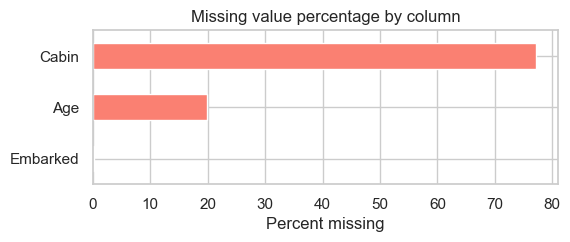
\includegraphics[width=0.7\textwidth]{missing_data.png}
    \caption{Missing data percentage by columns}
\end{figure}

\subsection{Correlation Analysis}
The correlation heatmap reveals links between numerical variables. There's a negative correlation between passenger class and survival, which suggests that first-class passengers had better survival rates. Fare is positively correlated with survival, showing the influence of socioeconomic status.
Other features, like number of siblings/spouses aboard and number of parents/children aboard, have relatively weak relationships with survival, implying they don't individually predict survival well.


\begin{figure}[H]
    \centering
    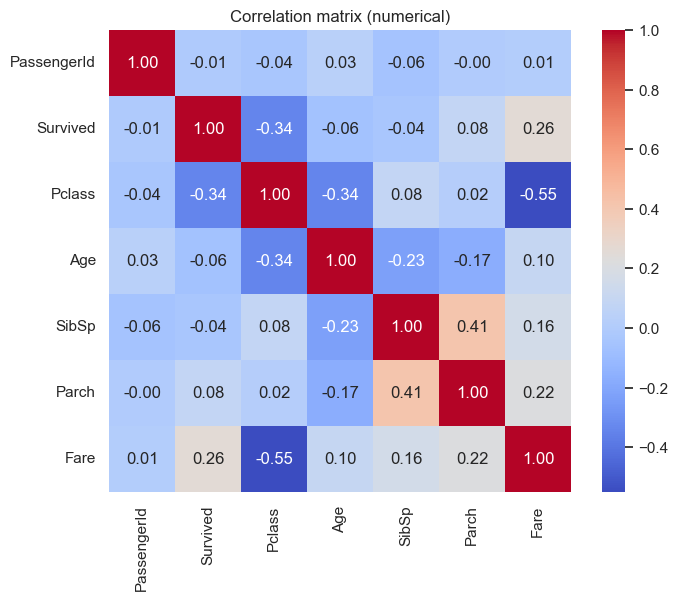
\includegraphics[width=0.7\textwidth]{correlation.png}
    \caption{Correlation heatmap on numerical features}
\end{figure}

\subsection{Age Distribution}
The age range of most passengers was 20–40 years. The data is a bit skewed to the right, meaning there were not as many older passengers. Because some age data was missing, we had to fill in those gaps before we could do the analysis.
This age range suggests most passengers were working adults.

\begin{figure}[H]
    \centering
    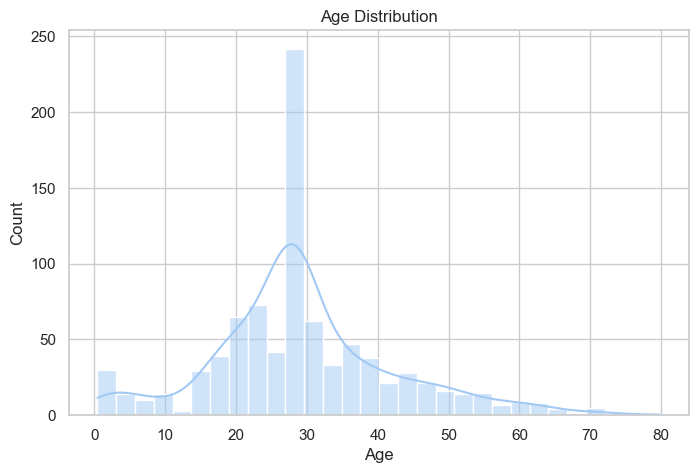
\includegraphics[width=0.63\textwidth]{age_distribution.png}
    \caption{Age distribution}
\end{figure}

\subsection{Fare Distribution}
The distribution of fares tends to be right-skewed, meaning a large percentage of riders pay lower fares, while a smaller percentage pay much higher fares. This skew suggests an economic difference between riders and backs the theory that passenger class affects ticket costs.

\begin{figure}[H]
    \centering
    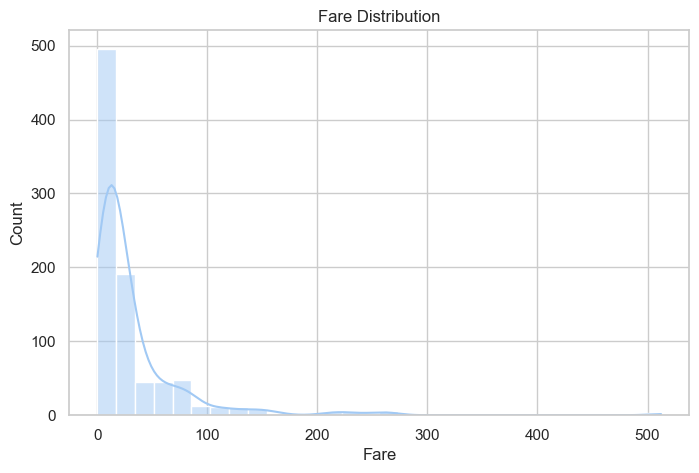
\includegraphics[width=0.63\textwidth]{fare_distribution.png}
    \caption{Fare distribution}
\end{figure}

\subsection{Age Distribution by Survival}
Children tend to survive at higher rates when age groups are compared with survival. Still, because the survivor and non-survivor groups share traits, age alone may not decide survival.

\begin{figure}[H]
    \centering
    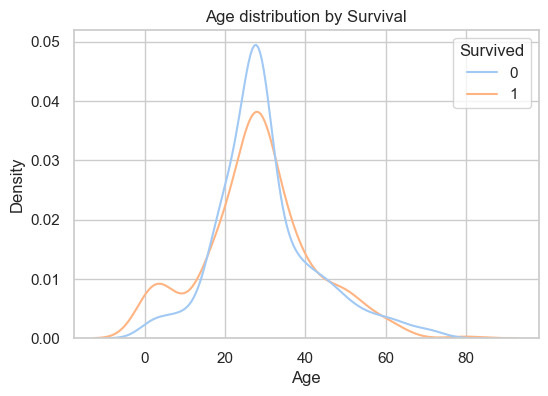
\includegraphics[width=0.65\textwidth]{age_dist_survival.png}
    \caption{Age distribution by Survival}
\end{figure}

\subsection{Overall Survival Distribution}
The survival rate shows that less than half of the passengers lived. This imbalance in the data should be considered in future predictive models and might need resampling methods.

\begin{figure}[H]
    \centering
    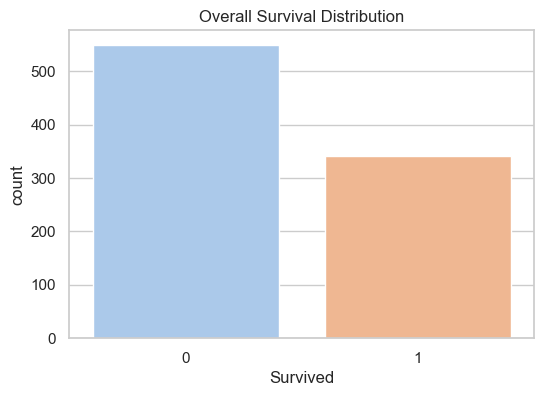
\includegraphics[width=0.6\textwidth]{survival_dist.png}
    \caption{Overall survival distribution}
\end{figure}


\subsection{Survival by Gender}
Gender is revealed to be one of the most significant predictors of survival. The survival rate of female passengers was significantly higher than that of males. This is not surprising, as the "women and children first" evacuation order has long been a tradition.\begin{figure}[H]
    \centering
    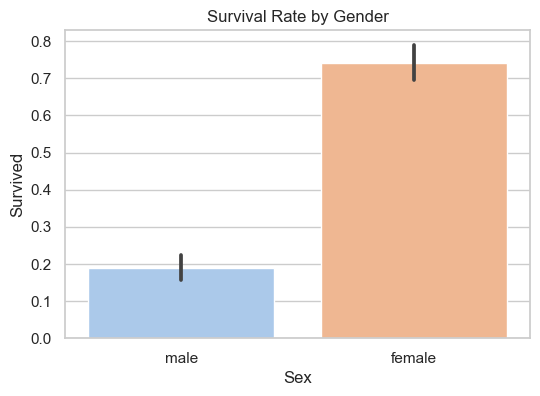
\includegraphics[width=0.55\textwidth]{survival_by_gender.png}
    \caption{Survival by gender}
\end{figure}

\subsection{Survival Rate by Passenger Class}
Passenger class was a very important factor in survival probability. The survival rate was highest among first-class passengers, followed by second-class passengers, while third-class passengers had the lowest survival rates.
This indicates that socioeconomic factors were a very important determinant, possibly because of their location in the cabin and easy access to the lifeboats.


\begin{figure}[H]
    \centering
    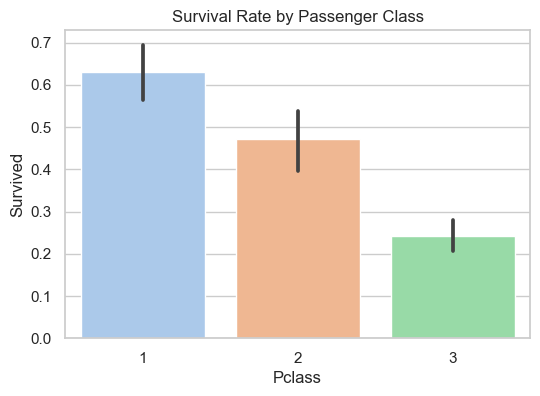
\includegraphics[width=0.55\textwidth]{survival_passenger_class.png}
    \caption{Survival Rate by Passenger Class}
\end{figure}

\subsection{Survival Rate by Embarkation Port}
The survival rates of passengers leaving Cherbourg were higher than those leaving Southampton and Queenstown. Given that many first-class passengers boarded at Cherbourg, this might be an indication of underlying class distributions.

\begin{figure}[H]
    \centering
    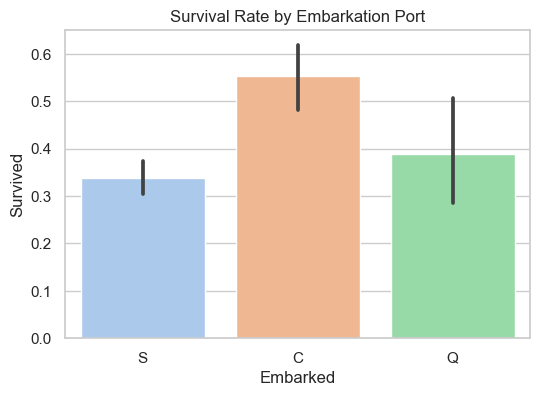
\includegraphics[width=0.5\textwidth]{survival_by_embarked.png}
    \caption{Survival Rate by Embarkation Port}
\end{figure}

\subsection{Survival Rate by Class and Gender}
Interaction effects are revealed when passenger class and gender are combined. The survival probability was lowest for third-class males and highest for first-class females. This demonstrates that socioeconomic status and gender had a combined impact on survival outcomes.

\begin{figure}[H]
    \centering
    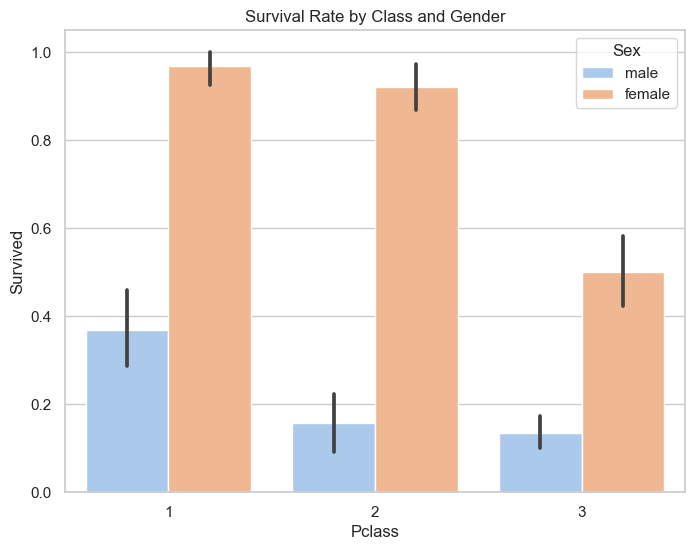
\includegraphics[width=0.5\textwidth]{survival_class_gender.png}
    \caption{Survival Rate by Class and Gender}
\end{figure}

\subsection{Survival Rate by Embarked and Gender}
Female survival rates were consistently higher than male survival rates at all embarkation ports. Nonetheless, there was a slight variation in the size of survival differences by port.

\begin{figure}[H]
    \centering
    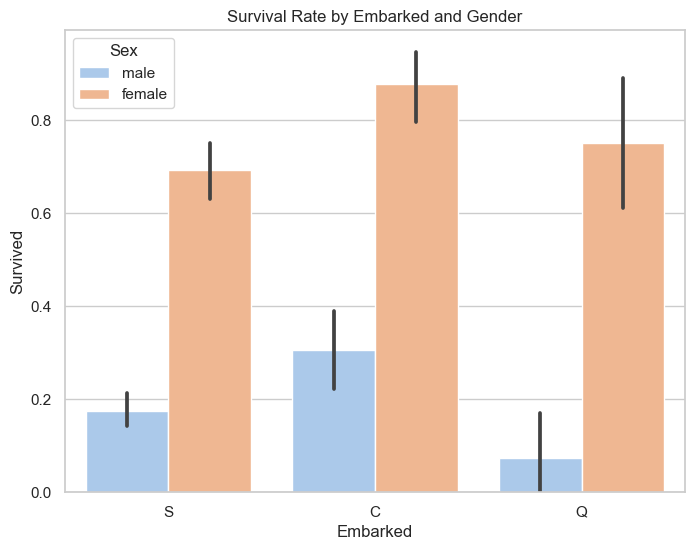
\includegraphics[width=0.7\textwidth]{survival_embarked_gender.png}
    \caption{Survival Rate by Embarked and Gender}
\end{figure}

\subsection{Survival Rate by Family Size}
To understand how family size affects survival, a new variable was made by putting together siblings/spouses (SibSp), parents/children (Parch), and the passenger. We found that passengers in small families (2–4 people) were more likely to survive than those who traveled alone or in big families. People who traveled alone had a fair chance of survival, but bigger families had organization problems that lowered their survival chances. In general, there was not a straight relationship between family size and how likely someone was to survive, which shows that being in a middle-sized group was helpful.

\begin{figure}[H]
    \centering
    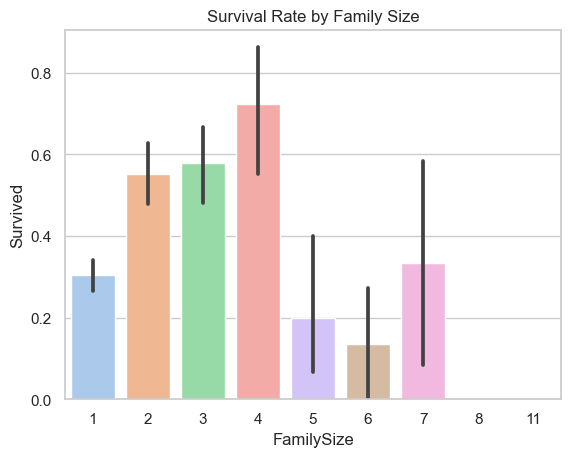
\includegraphics[width=0.55\textwidth]{survival_family.png}
    \caption{Survival Rate by Family Size}
\end{figure}


\subsection{Survival Rate by Age Group}
To study how age affected survival, passengers were put in groups: Child, Teen, Young Adult, Adult, and Senior. This made it easier to compare survival rates across different ages. The data showed kids survived more often than grown-ups and older people, which fits with stories of saving younger people first during the evacuation. Though age mattered, gender or money seemed to have a bigger impact on who survived. This means other things were probably more important.

\begin{figure}[H]
    \centering
    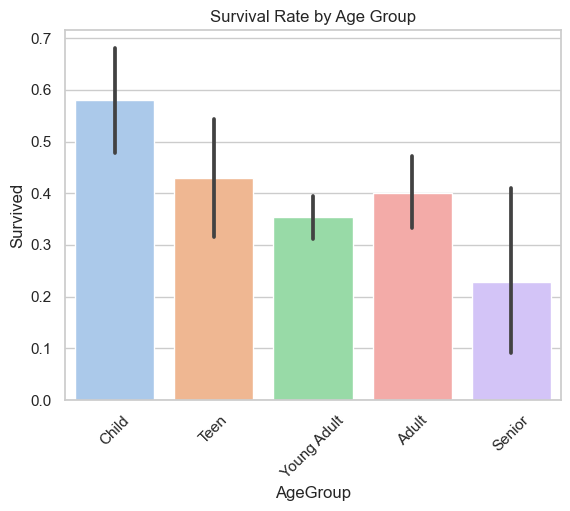
\includegraphics[width=0.55\textwidth]{survival_age_group.png}
    \caption{Survival Rate by Age Group}
\end{figure}



\section{Conclusion}
The exploratory data analysis of records from 891 passengers aboard the Titanic from the dataset \cite{1} pinpoints key factors that shaped survival during the disaster. Gender and passenger class appear as major factors; women and first-class passengers had much better chances of survival. Fare price also had a tie to survival, confirming the role of economic status. Age played a part. Children had higher survival rates than others, but it was not as large a factor as gender or class. Family size also mattered as passengers in smaller groups did better than those who were alone or in big families. To summarize, survival was dependent on social standing and economic factors. 

\begin{thebibliography}{99}

\bibitem{b1} S. Xu, "Titanic: Machine Learning from Disaster," Kaggle, 2023. [Online]. Available: \url{https://www.kaggle.com/datasets/shuofxz/titanic-machine-learning-from-disaster}. [Accessed: 7 Feb. 2026]. 

\end{thebibliography}

\end{document}
